\section{Overbelægning}

\subsection{Udvikling og betydning af overbelægning}
Overbelægning opstår, når en afdeling har flere indlagte patienter end sengepladser. \citep{denstoredanskeordbog1}  Overbelægning er estimeret til 85\% af det samlede antal sengepladser. Sengepladserne på sygehusene i Danmark er fra 1996 til 2011 reduceret med 30\%, for at tilnærme sig en udnyttelse af ressourcer på 100\%. \fxnote{nævn evt noget med underbelægning og at der skal være en balance mellem over- og underbelængning}
\citep{Madsen2014}. 


\subsection{Overbelægning i Danmark}
Antallet af patienter, der indlægges varierer fra måned til måned, hvorfor tilgængeligheden af sengepladser ligeledes varierer. Dette gør sig gældende på flere forskellige afdelinger i Danmark, hvilket er illustreret på \autoref{fig:overbelaegning_ran}.
                   
\begin{figure}[H]
\centering
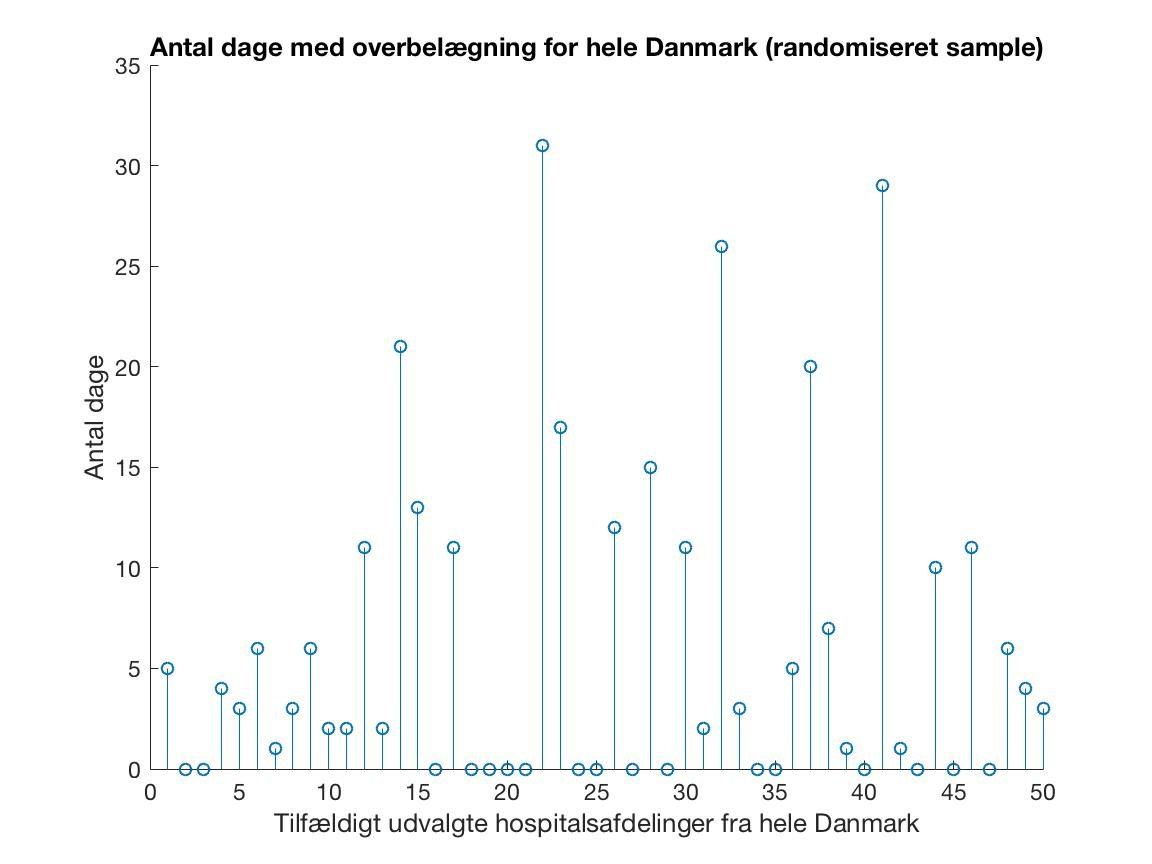
\includegraphics[width=1\textwidth]{figures/overbelaegning_ran.fig}
\caption{Antal dage med overbelægning udarbejdet med tilfældigt udvalgte hospitalsafdelinger fra hele Danmark. De randomiserede data er taget over januar måned i år 2015. \citep{SDS2015} \fxnote{uddyb figuren mere}} 
\label{fig:overbelaegning_ran}
\end{figure}

\noindent
Det ses af \autoref{fig:overbelaegning_ran}, at der er en tendens til overbelægning på flere hospitalsafdelinger i Danmark i forhold til underbelægning. Overbelægning strækker sig op til en måned. Det fremgår yderligere at der er en uligvægt mellem over- og underbelægning på de enkelte afdelinger. I de måneder hvor overbelægningen er størst, hvilket er januar til marts er overbelægningen på over 5 dage. Hvis der tages udgangspunkt i en enkelt afdeling understøttes det at der er et skel mellem over- og underbelægning.\citep{SDS2015} \fxnote{omskriv afsnit - det har ikke noget med underbelægning at gøre}

\begin{figure}[H]
\centering
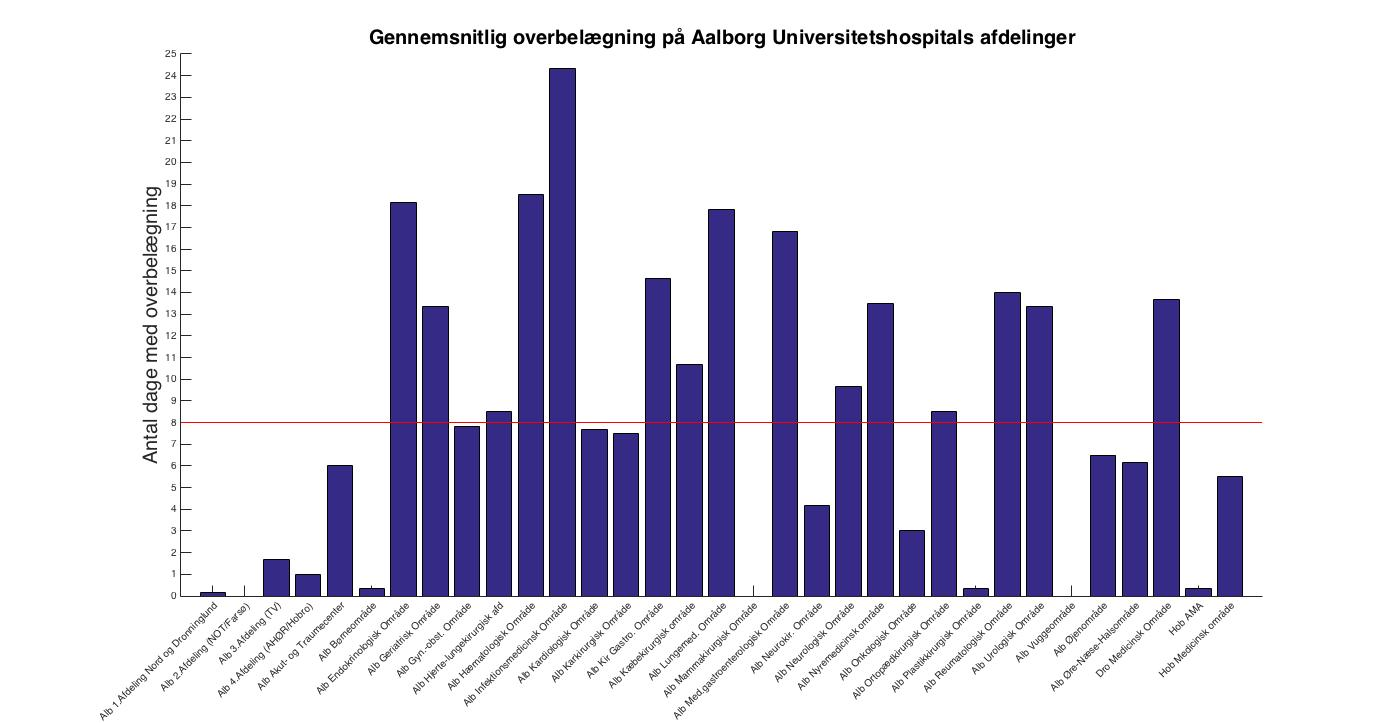
\includegraphics[width=1\textwidth]{figures/overbelaegning_AUH.fig}
\caption{Gennemsnitlig overbelægning på Aalborg Universitetshospitalsafdelinger målt i antal dage. Målingerne er taget for samtlige afdelinger på Aalborg Universitetshospital og er taget fra januar til juni i år 2015.\citep{SDS2015} \fxnote{omskriv og udddyb det med gennemsnit}}
\label{fig:overbelaegning_AUH}
\end{figure}

\noindent
Det fremgår af \autoref{fig:overbelaegning_AUH}, at den gennemsnitlige overbelægning på Aalborg Universitetshospital strækker sig op til 24 dage. \fxnote{skrives om ift grafen, nævn om forskellig grad. og nævn kun 1 søjle af overbelægning} Overbelægninger er størst på ambulatorisk infektionsmedicinsk område, ambulatorisk hæmatologisk område og ambulatorisk endokirinologisk. Det fremgår yderligere, at der ingen overbelægninger er på ambulatorisk 2. afdeling, ambulatorisk mammakirugisk  område og ambulatorisk vuggeområde. Det ses desuden, at den gennemsnitlige overbelægning på samtlige afdelinger varer op til 8 dage.\fxnote{omskrives} 

graf over stigende/faldende overbelægning over år. 




